\section{Antenna Design 1 -- Monopole}
\fixme{Efficiency graph for all modes}
\fixme{S-parameter with tunable capacitor at \SI{0.3}{pF}}
\fixme{Bandwidth tables edit}
\begin{figure}[htbp]
    \centering
    \begin{subfigure}[b]{0.24\linewidth}
        \centering
        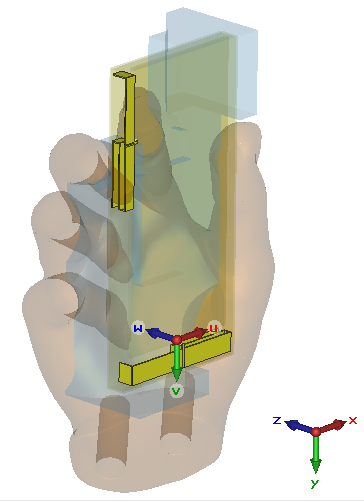
\includegraphics[width=\linewidth,height=4cm,keepaspectratio]{img/tech_sol/monopole/read_mode/3d_read_mode.PNG}
        \caption{Read mode.}
    \end{subfigure}
    \begin{subfigure}[b]{0.24\linewidth}
        \centering
        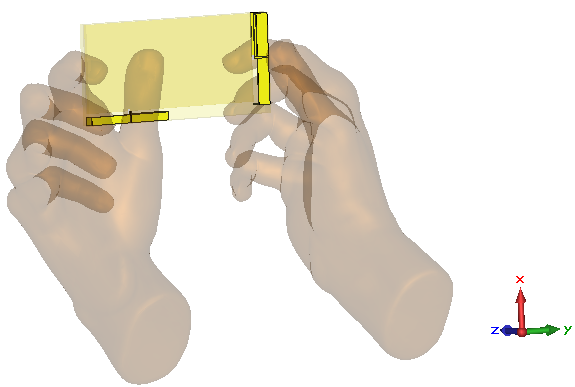
\includegraphics[width=\linewidth,height=4cm,keepaspectratio]{img/tech_sol/monopole/play_mode/3d_play_mode.PNG}
        \caption{Play mode.}
    \end{subfigure}
    \begin{subfigure}[b]{0.24\linewidth}
        \centering
        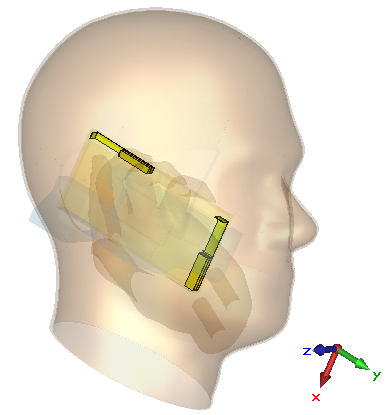
\includegraphics[width=\linewidth,height=4cm,keepaspectratio]{img/tech_sol/monopole/talk_mode/3d_talk_mode.PNG}
        \caption{Talk mode.}
    \end{subfigure}
    \begin{subfigure}[b]{0.24\linewidth}
        \centering
        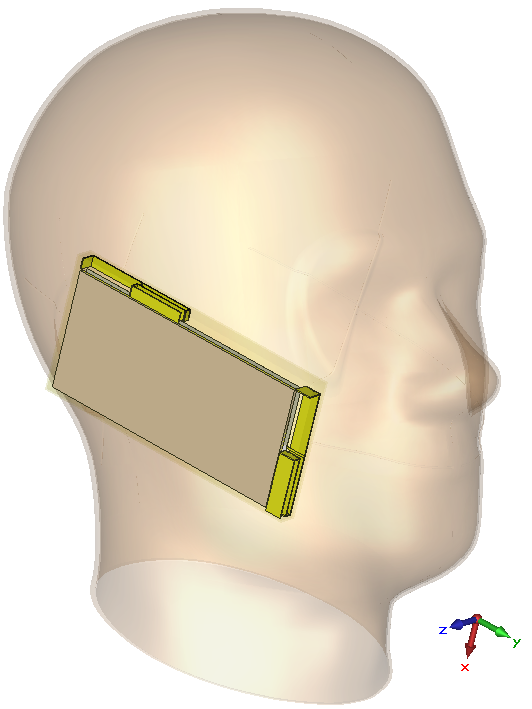
\includegraphics[width=\linewidth,height=4cm,keepaspectratio]{img/tech_sol/monopole/sar/3d_sar.PNG}
        \caption{SAR.}
    \end{subfigure}
    \caption{MIMO monopole antenna position for each user effect simulation.}
    \label{fig:sol1_monoant_positions}
\end{figure}


\subsection{Read Mode}

\begin{table}[htbp]
    \centering
    \begin{tabular}{|l|l|r|r|r|}
        \hline
        Antenna & Band & Start [MHz] & Stop [MHz] & Bandwidth [MHz] \\
        \hline
        Top     & Low  &          &        &  \\
        Side    & Low  &          &         &    \\
        \hline
        Top     & High &          &        &  \\
        Side    & High &         &        &  \\
        \hline
    \end{tabular}
    \caption{Monopole antenna in read mode. Maximum bandwidth obtained in the low and high band for the top and the side antenna, respectively.}    \label{tab:bw_sol1read}
\end{table}

\begin{figure}[htbp]
   \begin{subfigure}[b]{0.49\linewidth}
        \centering
        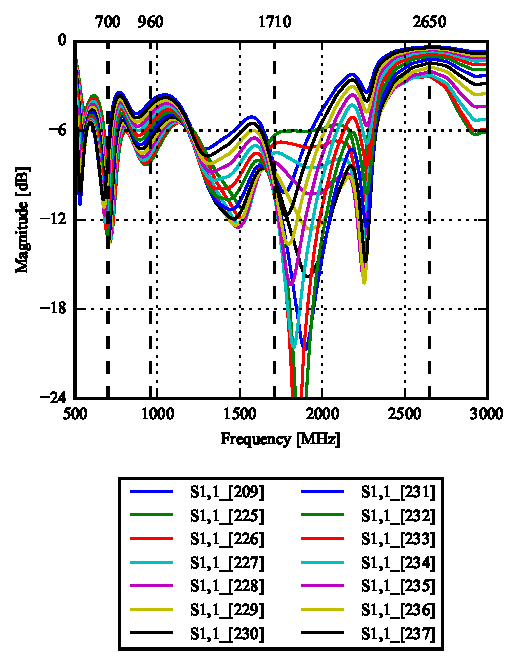
\includegraphics{img/tech_sol/monopole/read_mode/s11}
        \caption{$S_{11}$, sweeping $C_1$ and fixing $C_2$.}
    \end{subfigure}
    \hfill
    \begin{subfigure}[b]{0.49\linewidth}
        \centering
        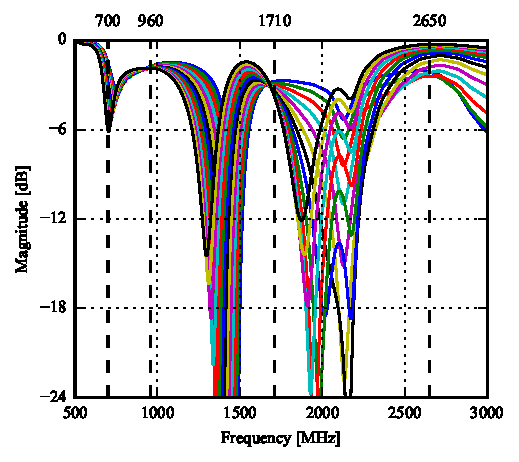
\includegraphics{img/tech_sol/monopole/read_mode/s22}
        \caption{$S_{22}$, sweeping $C_2$ and fixing $C_1$.}
    \end{subfigure}
~
    \begin{subfigure}[b]{0.49\linewidth}
        \centering
        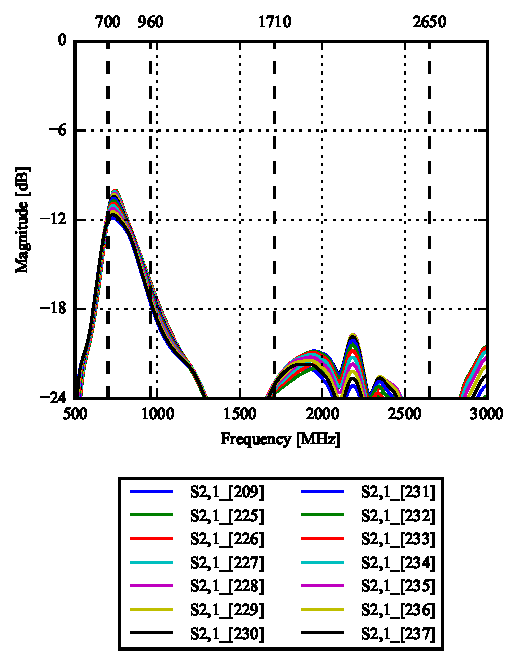
\includegraphics{img/tech_sol/monopole/read_mode/s21_s11}
        \caption{$S_{21}$, sweeping $C_1$ and fixing $C_2$.}
    \end{subfigure}
    \hfill
    \begin{subfigure}[b]{0.49\linewidth}
        \centering
        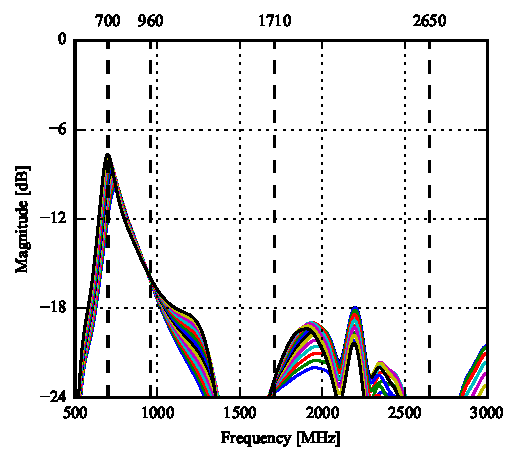
\includegraphics{img/tech_sol/monopole/read_mode/s21_s22}
        \caption{$S_{21}$, sweeping $C_2$ and fixing $C_1$.}
    \end{subfigure}
    \caption{Parameter sweep in read mode for tuning the shunt capacitor of each antenna, $C_1$ and $C_2$ for port 1 and 2, respectively. Port 1 is the top antenna and port 2 is the side antenna.}
    \label{fig:sparam_mono_read_mode}
\end{figure}

% Correlation
\begin{figure}[htbp]
    \centering
    \begin{subfigure}{0.49\linewidth}
        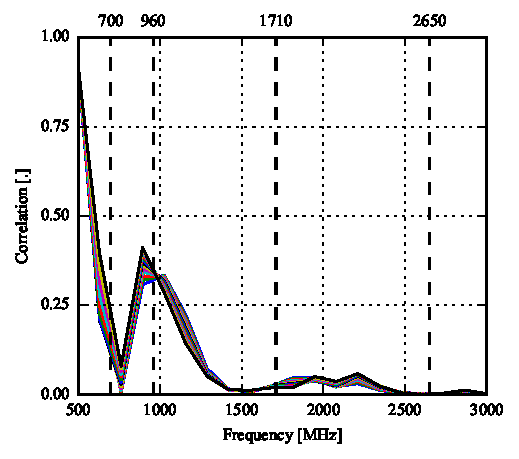
\includegraphics{img/tech_sol/monopole/read_mode/s11_corr}
        \caption{Sweeping $C_1$ and fixing $C_2$.}
    \end{subfigure}
    \hfill
    \begin{subfigure}{0.49\linewidth}
        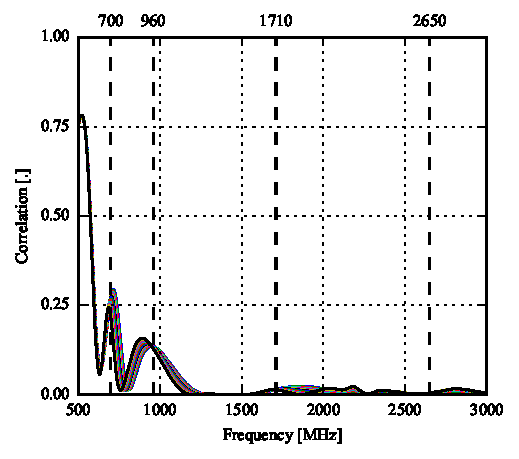
\includegraphics{img/tech_sol/monopole/read_mode/s22_corr}
        \caption{Sweeping $C_2$ and fixing $C_1$.}
    \end{subfigure}
    \caption{Monopole antenna in read mode. Correlation between antennas then sweeping tuning capacitors. Here, $C_1$ and $C_2$ are the tuning capacitor for the top and side antenna, respectively.}
    \label{fig:corr_sols_read}
\end{figure}

\subsection{Play Mode}

\begin{table}[htbp]
    \centering
    \begin{tabular}{|l|l|r|r|r|}
        \hline
        Antenna & Band & Start [MHz] & Stop [MHz] & Bandwidth [MHz] \\
        \hline
        Top     & Low  &          &        &  \\
        Side    & Low  &          &         &    \\
        \hline
        Top     & High &          &        &  \\
        Side    & High &         &        &  \\
        \hline
    \end{tabular}
    \caption{Monopole antenna in play mode. Maximum bandwidth obtained in the low and high band for the top and the side antenna, respectively.}    \label{tab:bw_sol1play}
\end{table}

\begin{figure}[htbp]
   \begin{subfigure}[b]{0.49\linewidth}
        \centering
        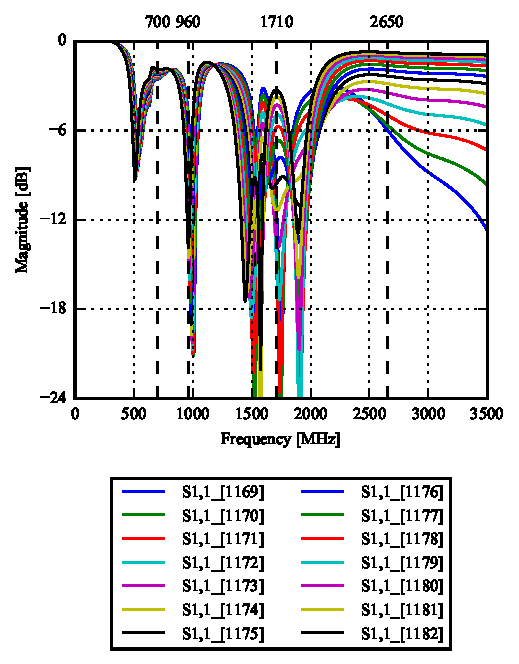
\includegraphics{img/tech_sol/monopole/play_mode/s11}
        \caption{$S_{11}$, sweeping $C_1$ and fixing $C_2$.}
    \end{subfigure}
    \hfill
    \begin{subfigure}[b]{0.49\linewidth}
        \centering
        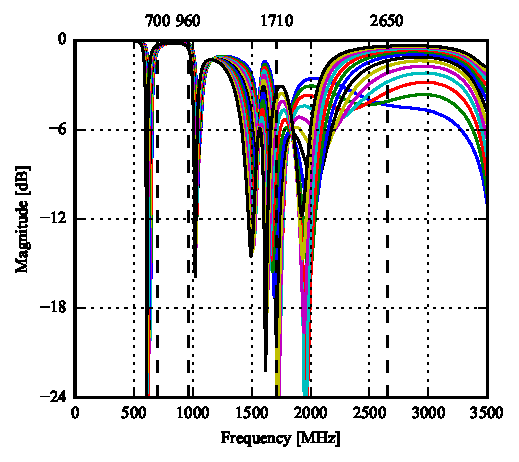
\includegraphics{img/tech_sol/monopole/play_mode/s22}
        \caption{$S_{22}$, sweeping $C_2$ and fixing $C_1$.}
    \end{subfigure}
~
    \begin{subfigure}[b]{0.49\linewidth}
        \centering
        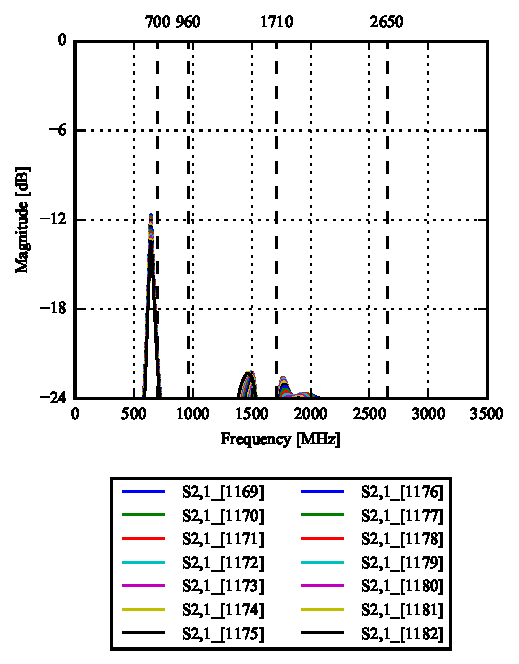
\includegraphics{img/tech_sol/monopole/play_mode/s21_s11}
        \caption{$S_{21}$, sweeping $C_1$ and fixing $C_2$.}
    \end{subfigure}
    \hfill
    \begin{subfigure}[b]{0.49\linewidth}
        \centering
        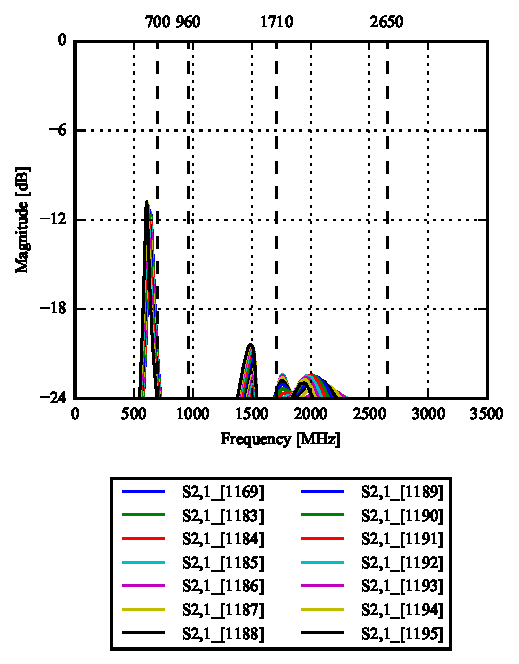
\includegraphics{img/tech_sol/monopole/play_mode/s21_s22}
        \caption{$S_{21}$, sweeping $C_2$ and fixing $C_1$.}
    \end{subfigure}
    \caption{Parameter sweep in play mode for tuning the shunt capacitor of each antenna, $C_1$ and $C_2$ for port 1 and 2, respectively. Port 1 is the top antenna and port 2 is the side antenna.}
    \label{fig:sparam_mono_play_mode}
\end{figure}

% Correlation
\begin{figure}[htbp]
    \centering
    \begin{subfigure}{0.49\linewidth}
        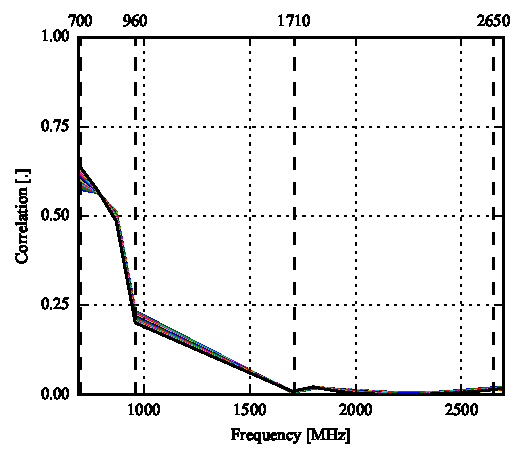
\includegraphics{img/tech_sol/monopole/play_mode/s11_corr}
        \caption{Sweeping $C_1$ and fixing $C_2$.}
    \end{subfigure}
    \hfill
    \begin{subfigure}{0.49\linewidth}
        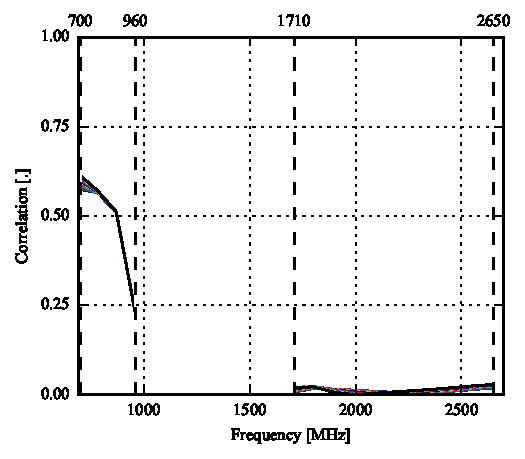
\includegraphics{img/tech_sol/monopole/play_mode/s22_corr}
        \caption{Sweeping $C_2$ and fixing $C_1$.}
    \end{subfigure}
    \caption{Monopole antenna in play mode. Correlation between antennas then sweeping tuning capacitors. Here, $C_1$ and $C_2$ are the tuning capacitor for the top and side antenna, respectively.}
    \label{fig:corr_sol1_play}
\end{figure}

\subsection{Talk Mode}
%bandwidth
\begin{table}[htbp]
    \centering
    \begin{tabular}{|l|l|r|r|r|}
        \hline
        Antenna & Band & Start [MHz] & Stop [MHz] & Bandwidth [MHz] \\
        \hline
        Top     & Low  &          &        &  \\
        Side    & Low  &          &         &    \\
        \hline
        Top     & High &          &        &  \\
        Side    & High &         &        &  \\
        \hline
    \end{tabular}
    \caption{Monopole antenna in talk mode. Maximum bandwidth obtained in the low and high band for the top and the side antenna, respectively.}    \label{tab:bw_sol1talk}
\end{table}

\begin{figure}[htbp]
   \begin{subfigure}[b]{0.49\linewidth}
        \centering
        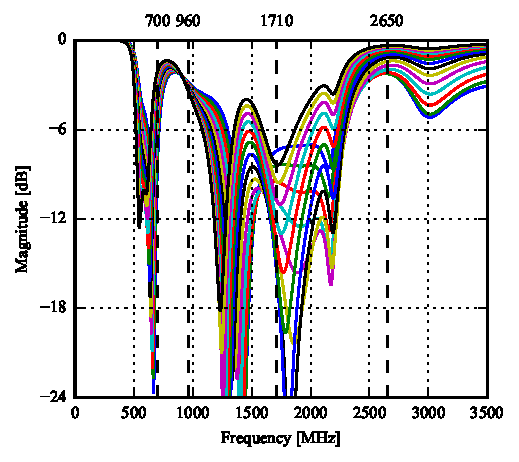
\includegraphics{img/tech_sol/monopole/talk_mode/s11}
        \caption{$S_{11}$, sweeping $C_1$ and fixing $C_2$.}
    \end{subfigure}
    \hfill
    \begin{subfigure}[b]{0.49\linewidth}
        \centering
        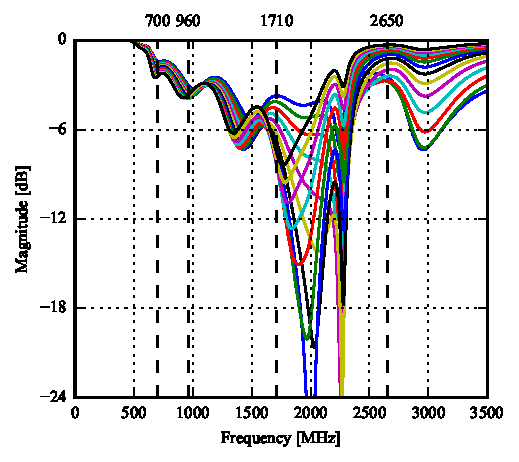
\includegraphics{img/tech_sol/monopole/talk_mode/s22}
        \caption{$S_{22}$, sweeping $C_2$ and fixing $C_1$.}
    \end{subfigure}
~
    \begin{subfigure}[b]{0.49\linewidth}
        \centering
        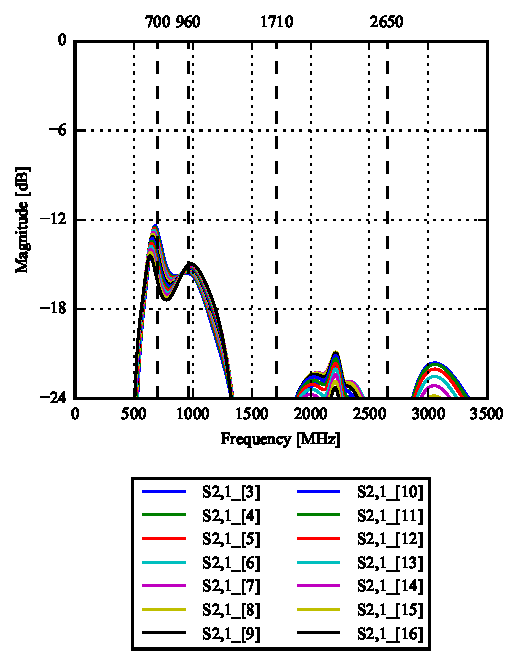
\includegraphics{img/tech_sol/monopole/talk_mode/s21_s11}
        \caption{$S_{21}$, sweeping $C_1$ and fixing $C_2$.}
    \end{subfigure}
    \hfill
    \begin{subfigure}[b]{0.49\linewidth}
        \centering
        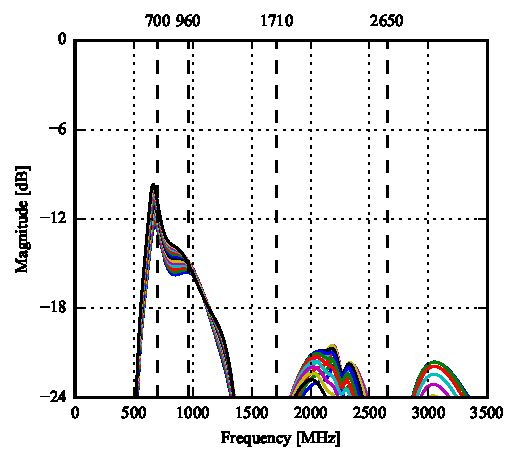
\includegraphics{img/tech_sol/monopole/talk_mode/s21_s22}
        \caption{$S_{21}$, sweeping $C_1$ and fixing $C_2$.}
    \end{subfigure}
    \caption{Parameter sweep for tuning the shunt capacitor of each antenna, $C_1$ and $C_2$ for port 1 and 2, respectively. Port 1 is the top antenna and port 2 is the side antenna.}
    \label{fig:sparam_mono_talk_mode}
\end{figure}
% Correlation
\begin{figure}[htbp]
    \centering
    \begin{subfigure}{0.49\linewidth}
        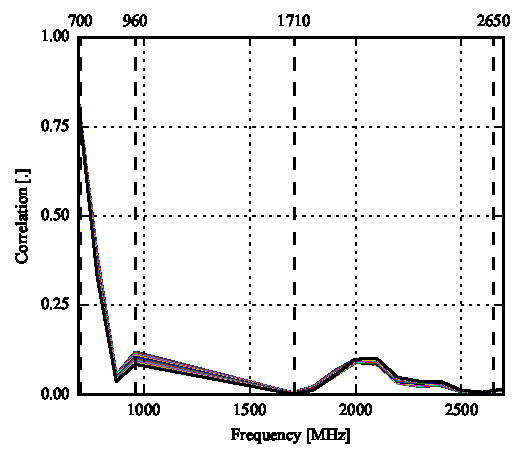
\includegraphics{img/tech_sol/monopole/talk_mode/s11_corr}
        \caption{Sweeping $C_1$ and fixing $C_2$.}
    \end{subfigure}
    \hfill
    \begin{subfigure}{0.49\linewidth}
        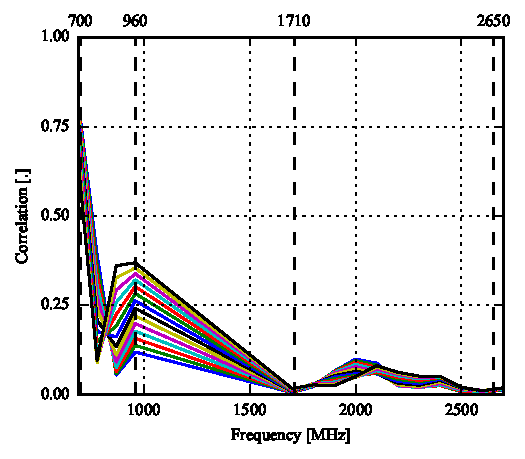
\includegraphics{img/tech_sol/monopole/talk_mode/s22_corr}
        \caption{Sweeping $C_2$ and fixing $C_1$.}
    \end{subfigure}
    \caption{Monopole antenna in read mode. Correlation between antennas then sweeping tuning capacitors. Here, $C_1$ and $C_2$ are the tuning capacitor for the top and side antenna, respectively.}
    \label{fig:corr_sol1_read}
\end{figure}

\subsection{SAR}

